%!TEX root = ../main.tex

\section{GCP Shielded VM (vTPM)}
%\addcontentsline{toc}{section}{GCP Shielded VM (vTPM)}


Shielded VM extends the concepts provided by Titan 
and brings them down to the guest (VM) OS Level, 
protecting end users from threats such as malicious UEFI drivers, 
boot vulnerabilities, and kernel vulnerabilities. 
The Shielded VM capabilities can be broken down into two main parts.

\subsection{Secure Boot}
Similar to Secure Boot with Titan, 
Shielded VM’s Secure Boot helps ensure that the system only runs authentic software 
by verifying the digital signature of all boot components on each boot.

\subsection{Measured Boot}
In a blog post\footnote{\url{https://cloud.google.com/blog/products/gcp/virtual-trusted-platform-module-for-shielded-vms-security-in-plaintext}} 
about TPMs, Google defines a TPM as 
“A TPM is a hardware, firmware, or virtual device that aids in securing machines 
in several ways: it can generate keys, use them for cryptographic operations 
(e.g., for symmetric and asymmetric key generation, signing, and decryption), 
and certify them based on its root Endorsement Key.” 
\citep{zimmerman_virtual_2018}.

The Shielded VM uses vTPM for Measured Boot, 
performing the measurements needed to create a known good boot baseline, 
called the integrity policy baseline. 
The integrity policy baseline validates that kernel and system drivers 
have not been tampered with, or rolled back to signed-but-unpatched binaries,
or load binaries out of order.

\begin{figure}[!ht]
    \centering
    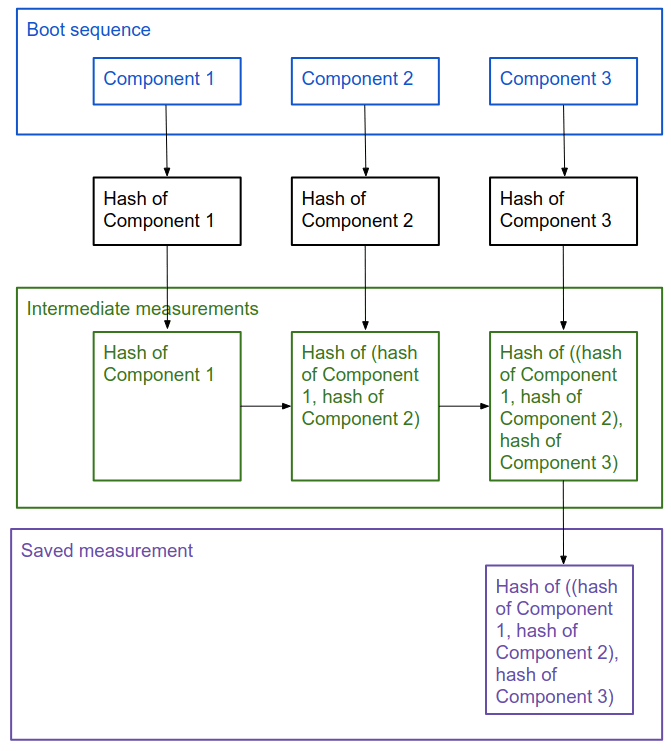
\includegraphics[width=0.5\linewidth]{measured-boot}
    \caption{Measured boot image from \cite{leibl_gcp_2022} and \cite{google_what_2022}}
    \label{fig:measured-boot}
\end{figure}


Measured Boot uses 
platform configuration registers\footnote{\url{https://link.springer.com/chapter/10.1007/978-1-4302-6584-9_12}} 
(PCRs) 
to store information about the components and component load order 
of both the integrity policy baseline 
(a known good boot sequence), 
and the most recent boot sequence 
\citep{arthur_platform_2015}.

\begin{figure}[!ht]
    \centering
    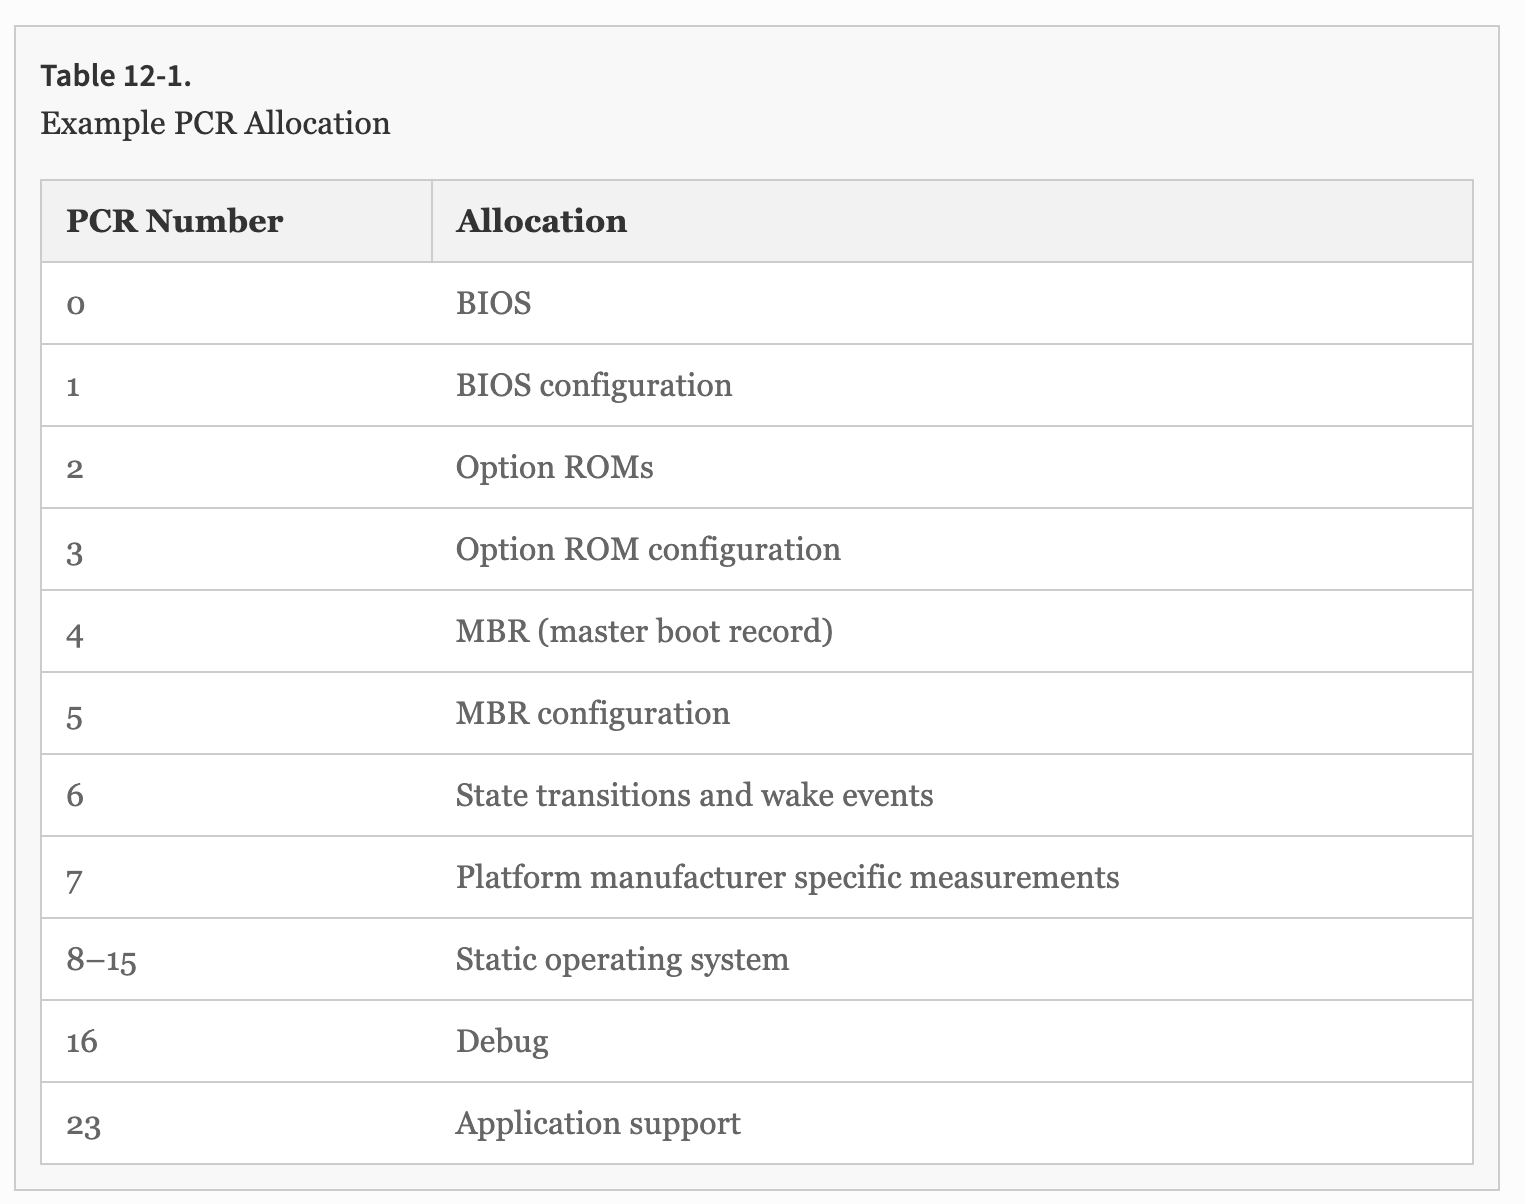
\includegraphics[width=0.6\linewidth]{configuration-registers}
    \caption{Configuration Registers image from \cite{arthur_platform_2015}}
    \label{fig:configuration-registers}
\end{figure}

\subsection{GCP VM Images}
The VM image that you use for your VM’s needs to support Shielded VM’s. 
The easiest way to achieve this is by using one of Google’s VM images. 
Alternatively you need to prepare a 
UEFI-compliant VM image\footnote{\url{https://cloud.google.com/compute/shielded-vm/docs/creating-shielded-images}} 
and store it on Google.

\subsection{GCP VM Log Events}
The typical event progression you see for your VM’s in the logs is startupEvent, 
earlyBootReportEvent, lateBootReportEvent, and eventually shutdownEvent, 
all with the same bootCounter value to identify them 
as describing the same VM instance boot sequence.

Shielded VM creates log entries for the following types of events:

\textbf{clearTPMEvent}\\
Identifies if the vTPM has been cleared, which deletes any secrets stored in it. 
This doesn't affect any aspect of the Shielded VM, 
so you will only care about this if you use the vTPM 
to shield sensitive data as described in vTPM\footnote{\url{https://cloud.google.com/compute/shielded-vm/docs/shielded-vm}} 
\citep{google_what_2022}.

\textbf{setShieldedInstanceIntegrityPolicy}\\
Logged each time you update the integrity policy baseline.

\textbf{shutdownEvent}\\
Logged each time the VM instance is stopped.

\textbf{startupEvent}\\
Logged each time the VM instance is started. 
The interesting information in this event is the bootCounter value, 
which identifies how many times this instance has been restarted.

\textbf{updateShieldedInstanceConfig}\\
Logged each time you enable or disable one of the Shielded VM options.

\textbf{earlyBootReportEvent}\\
Identifies whether the early boot sequence integrity check passed, 
and provides details on the PCR values from the baseline below,
the most recent boot sequence that were compared to make that determination.

\textbf{lateBootReportEvent}\\
Identifies whether the late boot sequence integrity check passed, 
and provides details on the PCR values from the baseline 
and the most recent boot sequence that were compared to make that determination.

\subsection{Determining the cause of boot integrity validation failure}
The actualMeasurements array contains the PCR values 
for the latest boot sequence. 
The values inside this array are compared to the policyMeasurements array 
to determine if there has been any change in the VM instance boot sequence. 
In the screenshot below PCR\_9 doesn’t match, which means the policy will fail.

\begin{figure}[!ht]
    \centering
    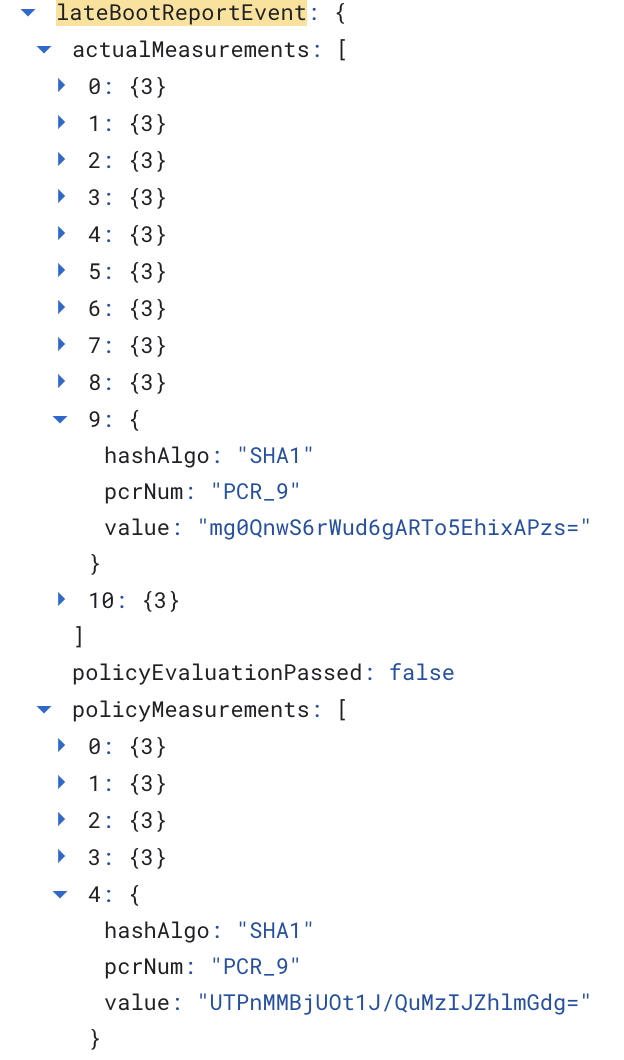
\includegraphics[width=0.3\linewidth]{pcr9}
    \caption{ PCR\_9 doesn’t match, which means the policy will fail.}
    \label{fig:pcr9}
\end{figure}

Sometimes, Shielded VM integrity measurements change for a \textbf{legitimate} reason. 
For example, a system update might cause expected changes to the operating system kernel. 
This is why every integrity failure should be investigated, whether the change is expected.